
\documentclass[11pt]{article}
\usepackage[margin=1in]{geometry}
\usepackage{graphicx}
\usepackage{amsmath}
\usepackage{hyperref}
\usepackage{caption}
\usepackage{booktabs}
\usepackage{array}
\usepackage{longtable}
\usepackage{fancyhdr}
\usepackage{titlesec}
\usepackage[numbers]{natbib}

\title{Designing Tools for Co-exploration: A Guideline to Support Remote Design Collaboration}

\author{
\begin{minipage}[t]{0.3\textwidth}
\centering
Xinhui Ye \\
Department of Industrial Design \\
Eindhoven University of Technology \\
\texttt{x.ye@tue.nl}
\end{minipage}
}

\date{}

\begin{document}

\maketitle

\begin{abstract}
Co-exploration is best understood not as a specific type of activity, but as an emergent experience that arises when design team members collaboratively engage in a shared design task. These moments of co-exploration can occur across various design stages and are often accompanied by a sense of togetherness that enables collective intelligence, allowing outcomes that no individual could achieve alone. Supporting co-exploration in remote settings is challenging, as the conditions that foster it, such as physical proximity, context awareness, and informal interaction, are often diminished. To address this, we developed the “Designing Tools for Co-exploration” (DTC) guideline as part of a study on remote design collaboration. Originally included as an appendix in the INTERACT 2025 paper “When Design Collaboration Goes Remote,” the DTC guideline captures intermediate-level design knowledge derived from expert interviews. Organized around three collaborative spaces — meeting space, working space, and project-specific space — the guideline articulates how people, materials, and interactions must coordinate to support co-exploration. It offers concrete design considerations and illustrative examples to guide the development of design tools and to support reflective practice within remote collaborative design teams.

\end{abstract}

\section{Introduction}

Co-exploration plays an important role in collaborative design practices. It refers to the shared, emergent experience through which team members engage with design challenges together, merging insights, reflecting on existing materials, diverging to generate more ideas, or refining in ways that propel the design forward. While this experience is reported as significantly missing in remote collaboration \cite{ye2021adjusting}, our work takes a deeper look into how the conditions that support co-exploration might still be created when teams are not co-located.

Remote teams frequently struggle to maintain awareness of each other's work, coordinate effectively across disparate tools, and recreate the spontaneous communication that fosters deep collective engagement. Supporting co-exploration in such contexts requires more than digital replicas of co-located tools. It demands a careful focus on the social, material, and interactional conditions that shape how collaboration unfolds.

This article introduces the Designing Tools for Co-exploration (DTC) guideline, a structured set of design considerations developed to address this challenge. Based on expert insights, the guideline articulates how remote collaboration might better support the emergence of co-exploration. It was developed as part of a broader research effort investigating expert visions of future remote co-exploration. The full study has been accepted for publication at INTERACT 2025, but is not yet publicly available. While that paper details the study's methodology and findings, this article focuses specifically on the DTC guideline, its structure, content, and value for both tool developers and collaborative design teams. Rather than serving as a fixed checklist, the guideline is intended as a reflective resource: a prompt for designers and collaborators to examine how people, materials, and interactions are coordinated in their current practices, and to identify opportunities to strengthen remote co-exploration.

\section{Method}
\begin{figure}[h]
    \centering
    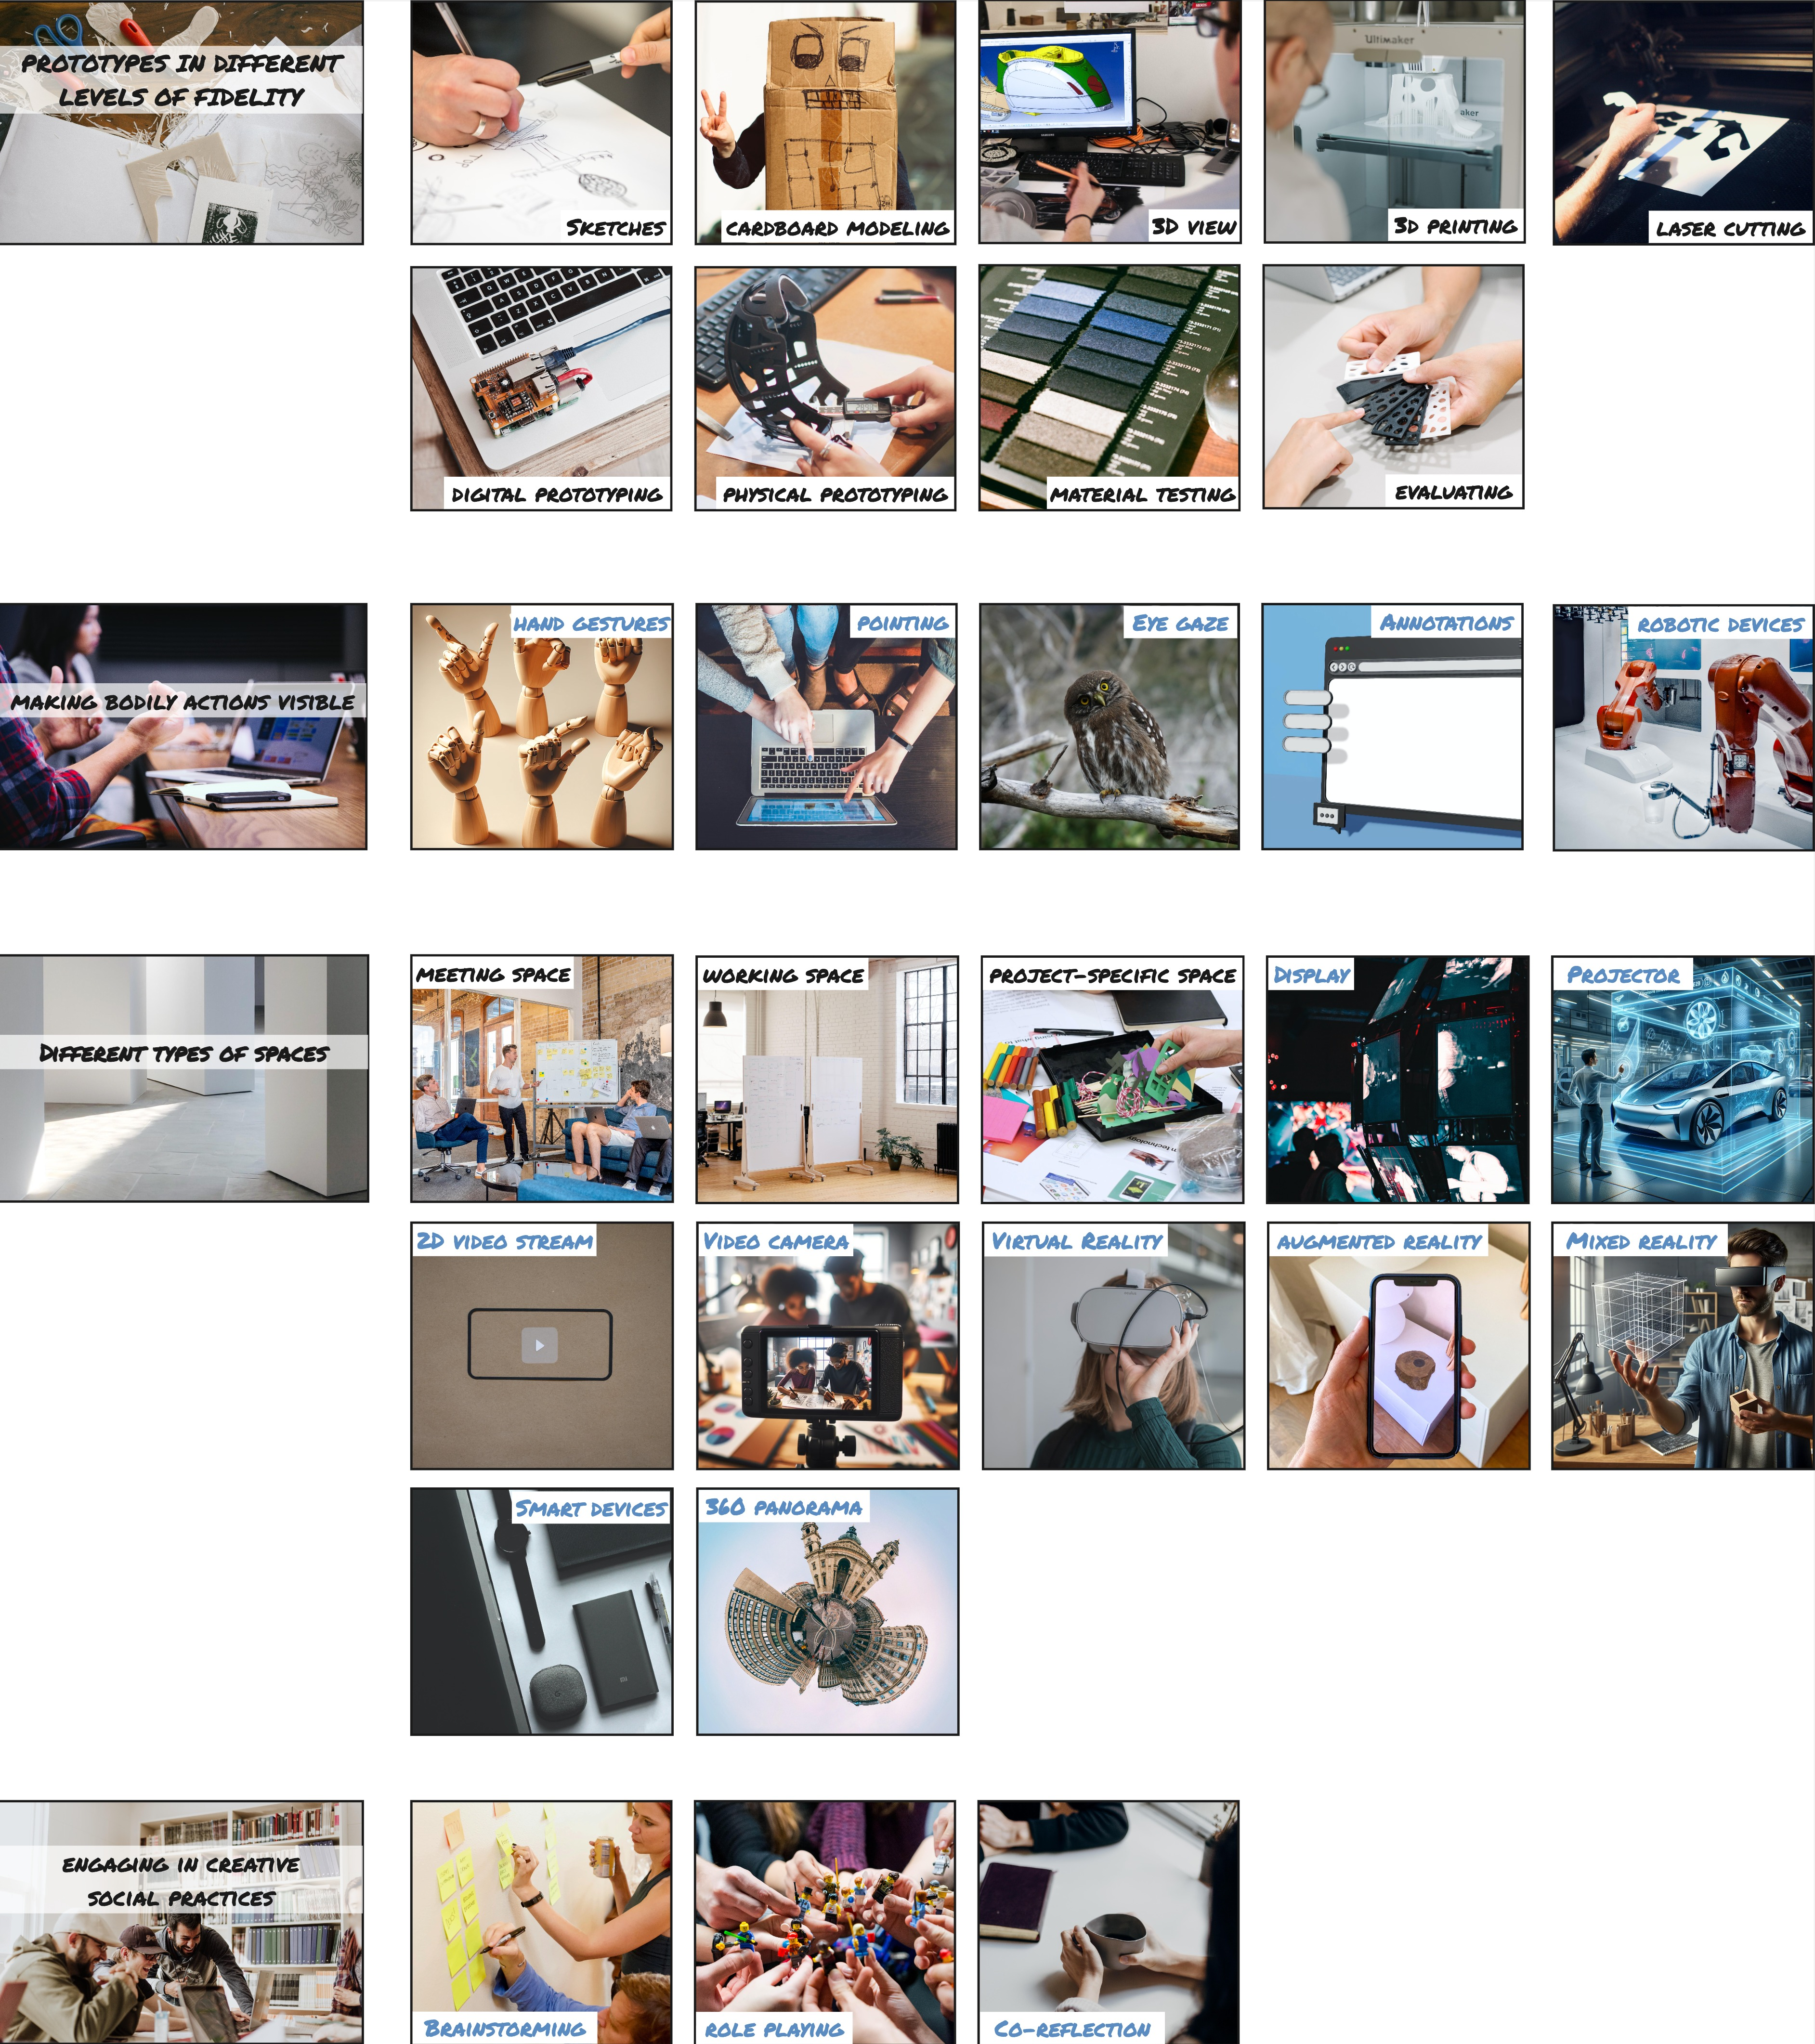
\includegraphics[width=0.7\linewidth]{figures/inspirational_cards.jpg}
    \caption{Overview of the full set of Inspirational Cards}
    \label{fig: inspirational cards}
\end{figure}

\noindent We invited eight professional design experts to share their experiences with co-exploration in both co-located and remote collaboration. Their insights informed a speculative design workshop aimed at envisioning how remote design tools might better support co-exploration.

To prompt reflection and inspire discussion, we created a set of inspirational cards (see Figure \ref{fig: inspirational cards}). These cards featured a mix of elements, including prototypes of varying fidelity, communication cues such as pointing, eye gaze, and hand gestures, as well as advanced technologies commonly explored in the field (e.g., augmented reality and robotic devices). During the sessions, participants used these cards as an inspirational resource to imagine new possibilities and concrete scenarios for enabling co-exploration at a distance.

Across all sessions, we collected approximately 15 hours of audio recordings and 22 posters, each containing fully formed design ideas. As illustrated in Figure \ref{fig: side talk}, one envisioned scenario describes a remote brainstorming session in which a team member’s eye gaze triggers a spontaneous side conversation, an interaction designed to replicate the informal exchanges typical in co-located work. To analyze the collected ideas,  we adapted the concept of annotated portfolios \cite{sauerwein2018annotated} as an instrument for interpreting the visual artifacts and discussions. Through this process, we synthesized the insights into the Designing Tools for Co-exploration (DTC) guideline. The guideline translates expert reflections into a set of structured design considerations, offering intermediate-level knowledge \cite{hook2012strong} intended to inform both the development of collaboration tools and the practices of distributed design teams.

The DTC guideline is organized around three collaborative spaces: meeting space, working space, and project-specific space. Within each, we identified recurring themes, key aspects to consider, and examples of design features or practices that can foster co-exploration remotely. 

\begin{figure}[h]
    \centering
    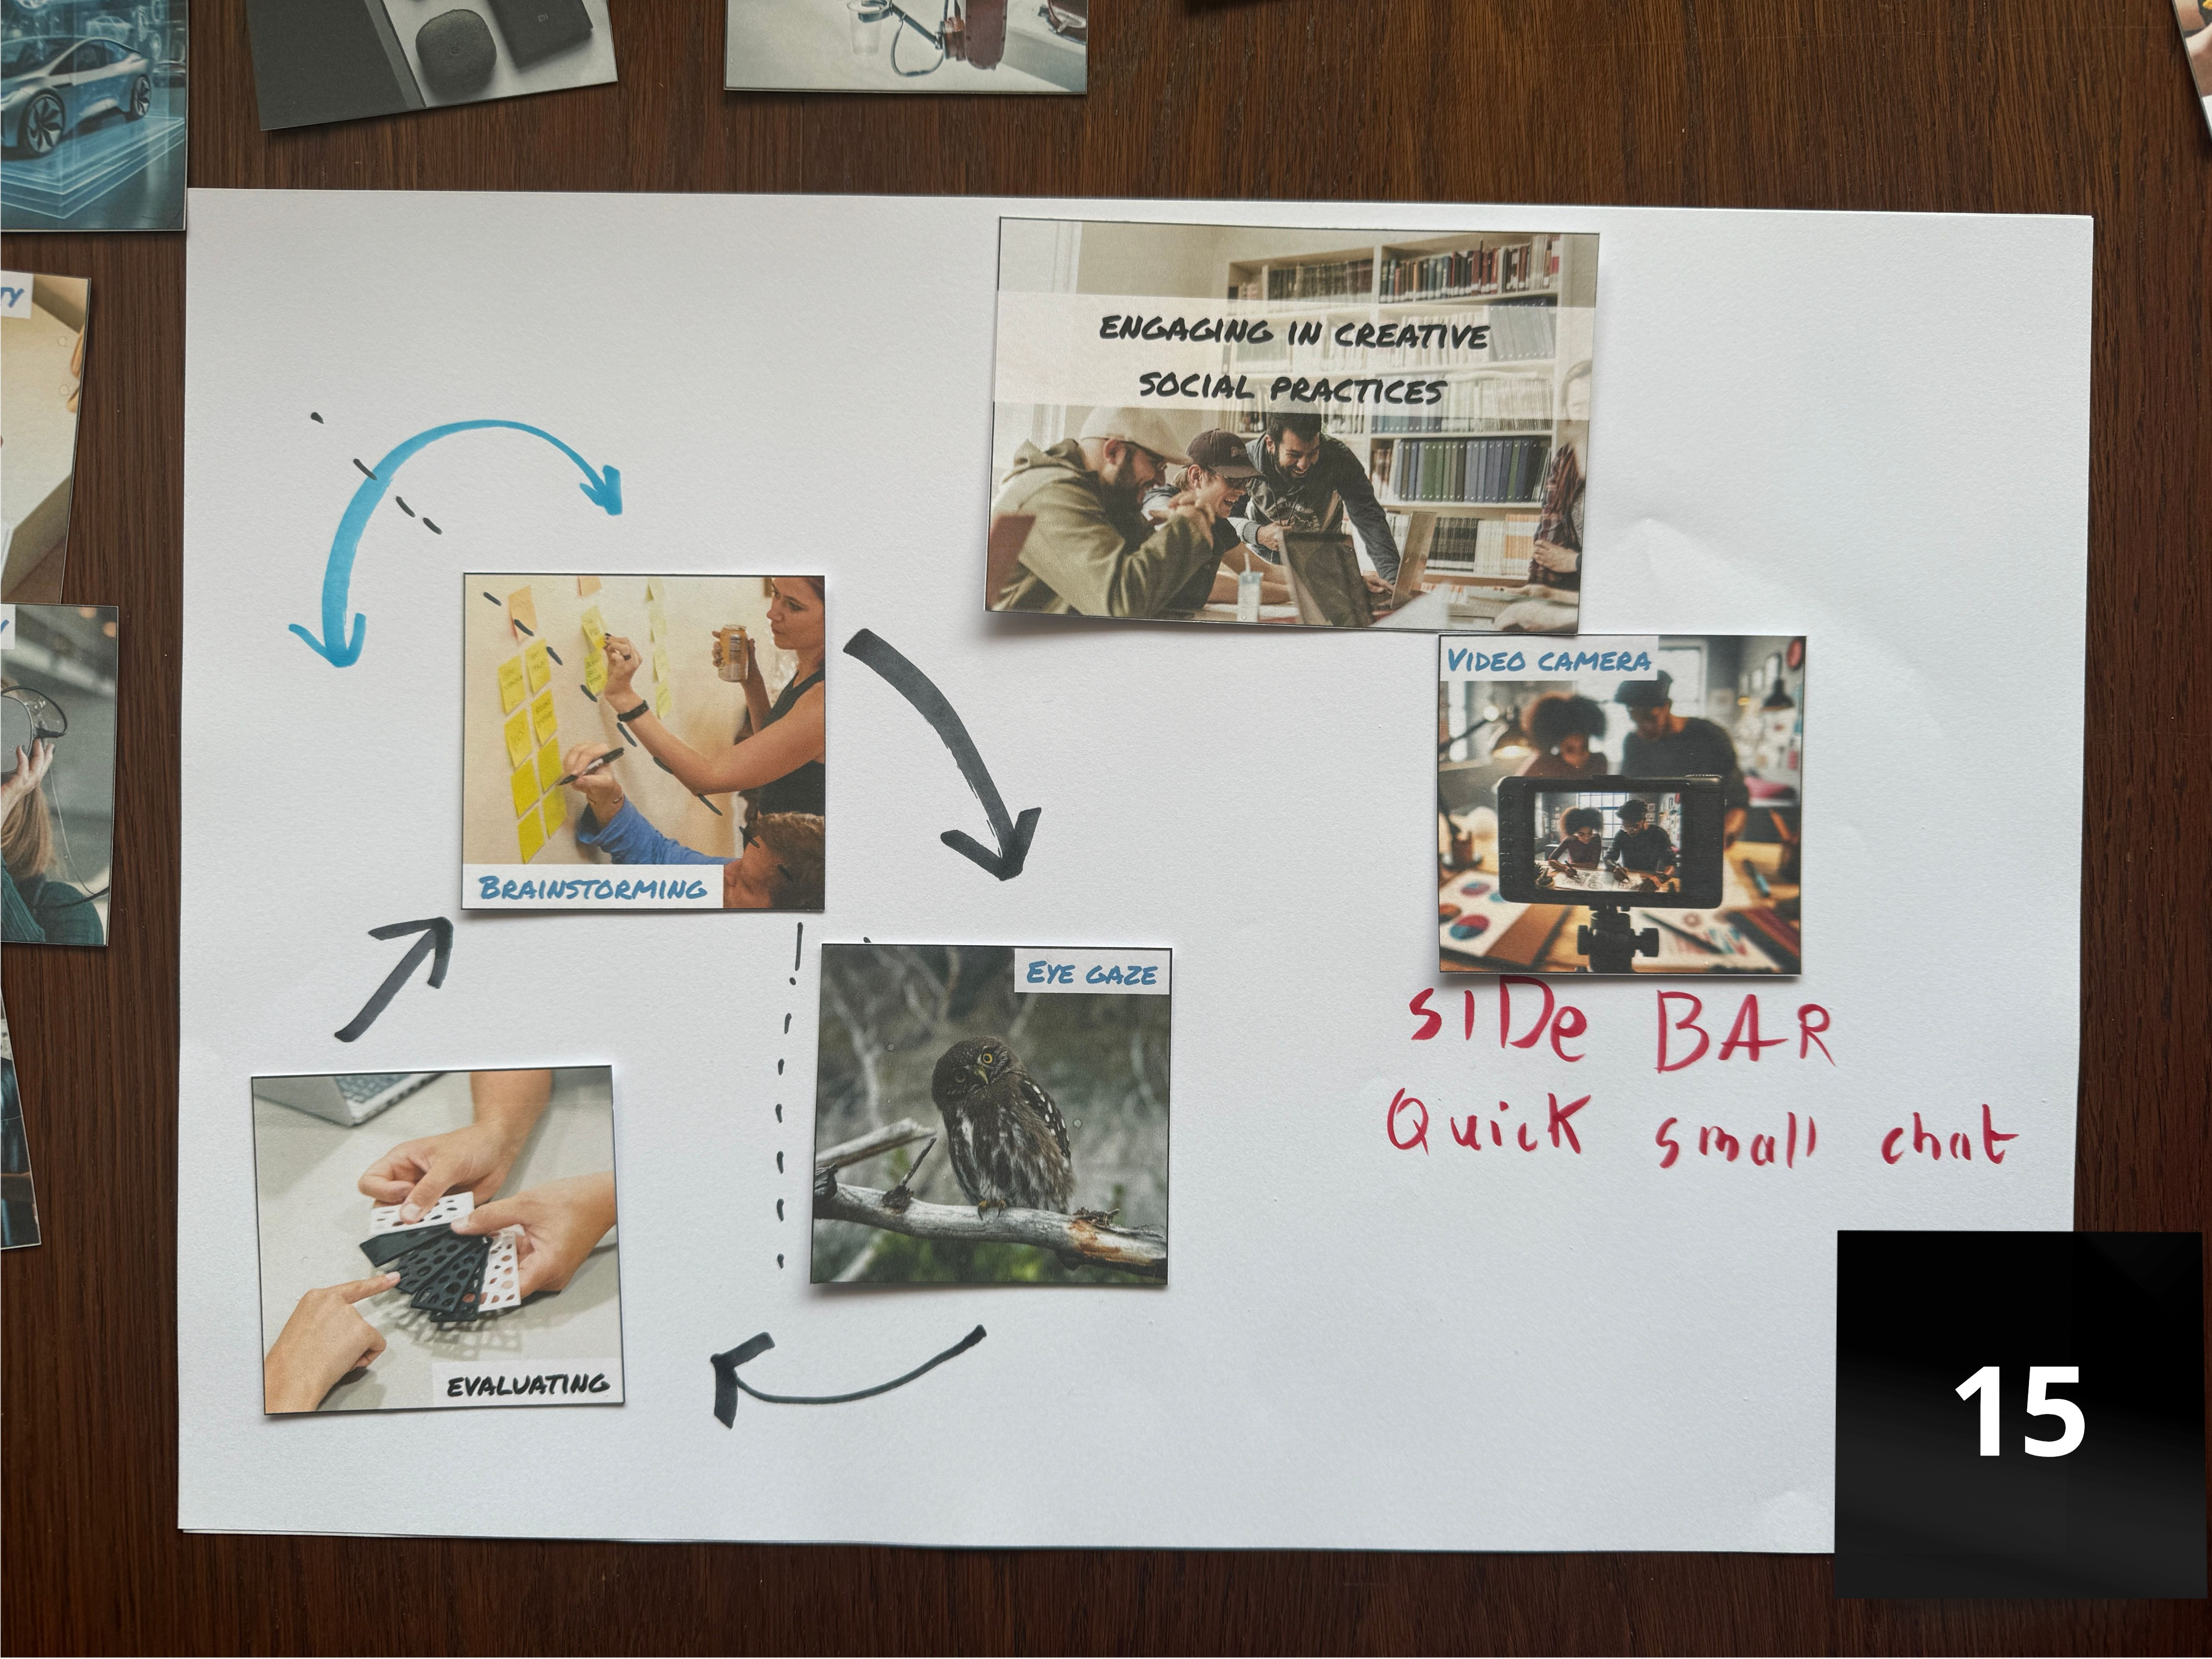
\includegraphics[width=0.7\linewidth]{figures/side_talk.jpg}
    \caption{Idea No.15: Using eye gaze to trigger a side conversation during brainstorming}
    \label{fig: side talk}
\end{figure}


\section {The DTC Guideline}
Rather than attempting to categorize activities by function or tool, we organized the guidelines around the situated contexts in which remote co-exploration could unfold. The three spaces, meeting, working, and project-specific, are conceptual spaces that help surface different design considerations. For example, informal communication that occurs in the working space may influence the awareness of ongoing work, thus shaping how shared materials are archived and revisited in the meeting space. This framing helped us map the nuanced interplay of people, materials, and interactions across settings. 

\begin{table}[ht]
\centering
\small
\caption{DTC guideline - Meeting Space}
\footnotesize
\begin{tabular}{|l|p{3.2cm}|p{4.5cm}|p{4.5cm}|}
\hline
\textbf{Theme} & \textbf{Key aspects} & \textbf{Considerations} & \textbf{Examples} \\
\hline

People & Contextual awareness of individual's work-in-progress 
& - How can collaborators be aware of the individual’s work-in-progress?
& - Improving the awareness from shared working space, e.g., Portholes\cite{dourish1992portholes} \newline - Creating logs for sharing each other’s work-in-progress (P3) \newline - Stand-up meetings, sprints\cite{stray2016daily} \newline - ... \newline {~}\\


{~} & Contextual awareness of project’s status 
& - How can collaborators be aware of the project’s status? \newline - How does it relate to the individual’s work-in-progress?
& - Improving the project-specific space for information sharing \newline - Stand-up meetings, sprints\cite{stray2016daily} \newline - ... \newline {~}\\


{~} & Individual preparation 
& - What information should be prepared in advance? \newline - How can this information be effectively shared?
& - Cloud-based file sharing, e.g., iCloud, Google Drive, etc. \newline - Fast shipment \newline - Rapid prototyping \newline - ... \newline {~}\\
\hline

Materials & Multi-fidelity prototypes 
& - What prototypes (e.g., sketches, paper models, CAD models, hi-fi prototypes) are needed for this co-exploration activity? \newline - What design elements (e.g., shape, scale, weight, texture, mechanisms, interactions) need to be explored?\newline {~}
& - Rapid prototyping \newline - Synchronized tool kit (P8) \newline - Sound effects for representing certain design elements (P6) \newline - ... \newline {~}\\


{~} & Accessibility and synchronization 
& - How can all collaborators access materials? \newline - How can prototypes be edited in real-time by all collaborators? \newline {~}
& - Robotic arms do prototype shaping (P1) \newline - Shared virtual space for design activities, e.g., Gravity Sketch\cite{Gravitysketch}, MIRIA\cite{buschel2021miria} \newline - ... \newline {~}\\
\hline

\end{tabular}
\end{table}


\clearpage
\begin{table}[ht]
\centering
\small
\caption{DTC guideline - Meeting Space}
\begin{tabular}{|l|p{3.2cm}|p{4.5cm}|p{4.5cm}|}
\hline
\textbf{Theme} & \textbf{Key aspects} & \textbf{Considerations} & \textbf{Examples} \\
\hline

Interactions & Group-based techniques 
& - What group-based design techniques are suitable for remote settings? \newline
- How can these techniques be effectively set up and facilitated? \newline
- How can breaks and individual work sessions be planned within these group-based activities? \newline
- What methods can be used to document and share the outcomes of group-based activities? \newline {~}
& - Shared whiteboard, e.g., Miro \newline
- DigitalDesk \cite{wellner1993digitaldesk}, MIRIA \cite{buschel2021miria} \newline
- Using AI to summarize the meeting content (P1) \newline
- ... \newline {~}\\


{~} & Maintaining enthusiasm and engagement 
& - How to mitigate the Zoom fatigue? \newline
- How to make online co-exploration activities more interactive?
& - Regular breaks (P3, P5) \newline
- Providing features for giving various types of feedback, e.g., reactions in Miro, Zoom polls, etc. \newline
- ... \newline {~}\\


{~} & Expressing and understanding the communication cues 
& - What are the appropriate communication cues (eye gaze, hand gestures, annotations, etc.) for different contexts? \newline
- How to express these communication cues remotely?
& - Better visibility of body language and facial expressions, e.g., CollaboVR \cite{he2020collabovr} and BeHere \cite{wang2023behere} \newline
- Avatars with real-time expression tracking, e.g., Apple Vision Pro \newline
- ... \newline {~}\\


{~} & Facilitating side conversation 
& - How can collaborators initiate side conversations during remote meetings? \newline
- How can these side talks be supported?
& - Eye gaze for triggering the function of side conversation (P8) \newline
- Breakout rooms \newline
- ... \newline {~}\\


{~} & AI-generated content 
& - How can AI tools assist in generating content to prompt further co-exploration activities? \newline
- How can AI be integrated into existing workflows without disrupting the co-exploration process? \newline {~}
& - Real-time AI-generated images for visualizing ideas during co-exploration (P8) \newline
- ... \newline {~}\\
\hline

\end{tabular}
\end{table}


\clearpage
\begin{table}[ht]
\centering
\small
\caption{DTC guideline - Working Space}
\begin{tabular}{|l|p{3.2cm}|p{4.5cm}|p{4.5cm}|}
\hline
\textbf{Theme} & \textbf{Key aspects} & \textbf{Considerations} & \textbf{Examples} \\
\hline

People & Informal Encounters 
& - How can tools support unplanned, spontaneous conversations in a way that mimics informal encounters in physical working environments? \newline {~}
& - Programmed meetups (P5) \newline
- In-situ information visualizations\cite{tang2001awarenex,monastero2018traces} \newline
- ... \newline {~}\\

{~} & Contextual awareness of an individual’s work-in-progress 
& - How can collaborators be aware of the individual’s work-in-progress? \newline
From where, through what, when?
& - Creating logs for sharing each other’s work-in-progress (P3) \newline
Portholes\cite{dourish1992portholes} \newline
- Using eye gaze to ‘zoom in’ to others’ individual space (P7) \newline
- ... \newline {~}\\
\hline

Materials & Ambient creative stimulus 
& - How can we transform the inspiring surroundings of a physical design studio into a remote setting? \newline {~}
& - Shared project-specific space \newline
- ... \newline {~}\\
\hline

Interactions & Informal social interactions 
& - How can collaborators indicate that they are open to informal interactions?
& - In-situ information visualizations\cite{tang2001awarenex,monastero2018traces} \newline
- ... \newline {~}\\


{~} & Maintaining togetherness 
& - What activities or routines can build a sense of togetherness, preventing collaborators from feeling isolated while working remotely?
& - Stand-up meetings, sprints\cite{stray2016daily} \newline
- Programmed meetups (P5) \newline
- Informal communication before and after formal meetings\cite{hu2022fluidmeet} \newline
- ... \newline {~}\\

{~}& Pre-meeting huddle 
& - How can pre-meeting discussions be organized to pave the way for addressing difficult problems?
& - Creating opportunities for informal social interactions (P1, P5) \newline
- ... \newline {~}\\

{~} & expressing, and understanding communication cues 
& - What are the appropriate communication cues (eye gaze, hand gestures, annotations, etc.) during interactions? \newline
- How to express these communication cues remotely?
& - Better visibility of body language and facial expressions, e.g., Cisco TelePresence or Microsoft Surface Hub \newline
- Avatars with real-time expression tracking, e.g., Apple Vision Pro \newline
- ... \newline {~}\\
\hline

\end{tabular}
\end{table}


\clearpage
\begin{table}[ht]
\centering
\small
\caption{DTC guideline - Project-specific space}
\begin{tabular}{|l|p{3.2cm}|p{4.5cm}|p{4.5cm}|}
\hline
\textbf{Theme} & \textbf{Key aspects} & \textbf{Considerations} & \textbf{Examples} \\
\hline

People & Contextual awareness of project’s status 
& - What indicators (e.g., progress bars, task status updates, milestone markers) could be included to give collaborators instant context about the project’s progress?
& - Dashboard presenting crucial indicators, e.g., Monday\cite{monday} \newline
- Summaries from the work logs (P3) \newline
- ... \newline {~}\\

{~} & Encouraging knowledge sharing 
& - How to motivate team members to actively share their work-in-progress?
& - Easy accessibility \newline
Focus on mastery rather than performance\cite{kim2017mosaic} \newline
- ... \newline {~}\\
\hline

Materials & Material archives for future reference 
& - How and where can collaborators store materials for future reference? \newline
- How can these materials be presented within their range of vision?
& - Shared desk/display for project-related materials (P6, P7) \newline
- ... \newline {~}\\


{~} & Accessibility and synchronization 
& - How can the materials and annotations in this space be synchronized across all collaborators?
& - Scanning and projecting (P7) \newline
- ... \newline {~}\\
\hline

Interactions & Traces of interactions with materials 
& - How can collaborators know and view interactions related to materials?
& - Video recording \newline
- Logs of all changes \newline
- ... \newline {~}\\
\hline

\end{tabular}
\end{table}

\section{Conclusion}

While the DTC guideline is grounded in expert reflections and ideations, it is not exhaustive. It is meant to be interpreted, adapted, and extended by those who use it. Future work could explore how the guideline performs when applied in live design settings or adapted for different domains. For now, it stands as a resource for teams and tool developers who seek to support more thoughtful, collaborative, and exploratory remote design work.

\newpage
\bibliographystyle{plainnat}
\bibliography{references}

\end{document}
